\documentclass[12pt]{article}
\usepackage[T1]{fontenc}
\usepackage[polish]{babel}
\usepackage[utf8]{inputenc}
\usepackage{lmodern}
\selectlanguage{polish}
\usepackage{graphicx}
\usepackage{mathtools}
\usepackage{spverbatim}
\usepackage{float}
\linespread{1.25}
\graphicspath{{/home/franek/Pictures/}}

\title{Praca magisterska}
\author{slupskifranek }
\date{May 2019}

\begin{document}

\maketitle


\section{Wstęp}

\subsection{Testowa baza danych}
Aby przedstawić techniki optymalizacji zawarte w pracy na rzeczywistych przykładach, wykorzystałem bazę danych udostępnioną przez portal stackoverflow.com. Baza zawiera w granicach 50 Gb danych zebranych w latach 2008-2013. Archiwum po zaimportowaniu do serwera MySQL nie zawiera klucz głównych, kluczy obcych, indeksów.
Początkowy schemat bazy danych jest przedstawiony na rysunku 1.
\begin{figure}
    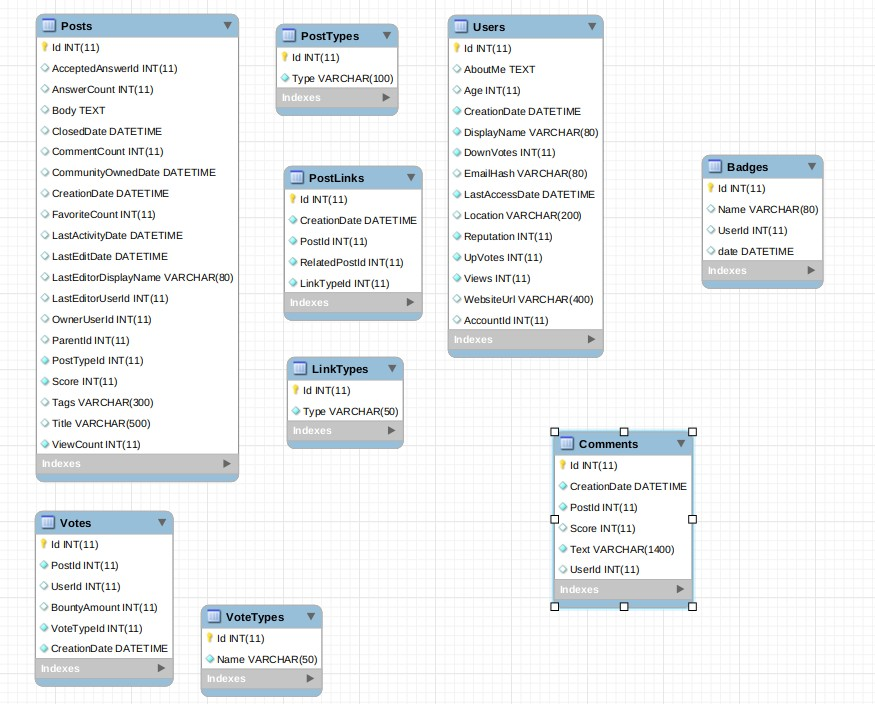
\includegraphics[scale =0.5]{schemat-baza-stackoverflow.jpg} 
    \caption{Schemat bazy danych stackoverflow}
\end{figure}



\subsection{Porównywanie zapytań}
W rozdziale zostanie przedstawione działanie polecenia EXPLAIN. Polecenie to umożliwia uzyskanie informacji o planie wykonania zapytania. Jest podstawowym sposobem określenia, w jaki sposób MySQL wykonuje zapytania. Analiza wyników EXPLAIN jest zdecydowanie bardziej użyteczna od mierzenia czasów zapytań. Na czas wykonania zapytania mogą mieć wpływ zewnętrzne czynniki, które wprowadzą nas w błąd podczas badania wydajności danego zapytania. Pierwszym z nich jest cache zapytań. Przeprowadzając testy zapytania przy włączonym buforze zapytań, może zdarzyć się, że rezultat zapytania zostanie zwrócony z tego właśnie bufora. Doprowadzi to do sytuacji, kiedy nawet najbardziej niewydajne zapytania będą zwracane w ułamek sekundy.  Problem ze zwracaniem wyników z bufora zapytań możemy rozwiązać poprzez wyłączenie bufora zapytań lub dodanie modyfikatora SQL\textunderscore NO\textunderscore CACHE do zapytań. Drugim czynnikiem zaburzającym mierzenie czasów wykonania zapytań jest bufor MySQL. MySQL stara się przechowywać w pamięci często używane dane, dla przykładu indeksy. Jeżeli wykonujemy zapytanie dla tabeli, której indeks nie znajduje się w pamięci. Serwer pobiera indeks z dysku, co trwa. Następnie poprawiamy zapytanie w celu poprawienia wydajności i wykonujemy, aby sprawdzić, czy nasze działanie poprawiło wydajność. Tym razem cały indeks znajduje się w pamięci i zapytanie wykonuje się wielokrotnie szybciej. Mierząc jedynie czasy wykonania obu zapytań, możemy dojść do fałszywego wniosku, że drugie zapytanie jest wydajniejsze, nawet jeżeli w rzeczywistości nasze działanie doprowadziło do pogorszenia wydajności zapytania. W takim przypadku dobrym rozwiązaniem wydaje się kilkukrotne mierzenie czasów, obliczenie średniej i na tej podstawie porównywanie wyników. Dodatkowo nasz serwer rzadko kiedy jest całkowicie odcięty od świata. Bardzo często będziemy testować wydajność zapytań na tabelach, które są w równocześnie modyfikowane w tle. Przykładowo jeżeli testujemy zapytanie na tabeli, na której równocześnie wykonywane są operacje zapisu, czasy wykonania naszego zapytania nie będą miarodajne. Dodatkowo na czasy wykonywania zapytań wpływ może mieć aktualne obciążenie serwera, co nie ułatwia pracy przy porównywaniu wyników. Jak widzimy aby skutecznie porównywać wydajność zapytań nie powinniśmy opierać się jedynie na czasie ich wykonania.
\subsection{Polecenie EXPLAIN}
Polecenie EXPLAIN będzie jedną z głównych metod porównywania wydajności zapytań stosowaną w tej pracy, dlatego w tym podroździale przedstawie podstawy stosowania tego polecenia. Funkcja EXPLAIN to główny sposób określania, jaki sposób wykonania zapytania wybrany na etapie jego optymalizacji przez optymalizator MySQL.

Aby użyć polecenia EXPLAIN, wystarczy poprzedzić słowa kluczowe takie jak SELECT,INSERT,UPDATE,DELETE poleceniem EXPLAIN. Spowoduje to, że zamiast wykonania zapytania, sewer zwróci informacje o planie wykonania. Rezultat polecenia EXPLAIN zawiera po jednym rekordzie dla każdej tabeli użytej w zapytaniu. Kolejność wierszy w wyniku zapytania odpowiada kolejności, w jakiej MySQL będzie wykonywał zapytania.  Pierwszym zapytaniem wykonanym przez MySQL będzie zapytanie z ostatniego wiersza.

\subsubsection{Wyniki polecenia EXPLAIN}
Żeby zademonstrować wyniki polecenia EXPLAIN na rzeczywistych przykładach wykonałem kilka zapytań EXPLAIN na bazie StackOverflow. Dla porządku uznajmy, że zapytania są ponumerowane względem kolejności ich występowania w rozdziale.
\begin{spverbatim}
	SELECT u.DisplayName, c.CreationDate, c.`Text` FROM  Comments c LEFT JOIN Users u ON c.UserId = u.Id WHERE c.PostId = 875;
\end{spverbatim}
\begin{figure}[H]
	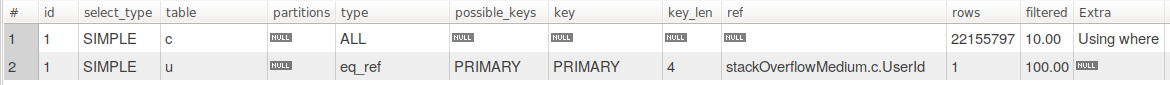
\includegraphics[scale =0.4]{explain7.png} 
	\caption{Przykład 1}
\end{figure}
\begin{spverbatim}
	SELECT p.Body FROM Posts p WHERE p.Id = 875 UNION
	SELECT c.`Text` FROM Comments c WHERE c.PostID = 875;
\end{spverbatim}
\begin{figure}[H]
	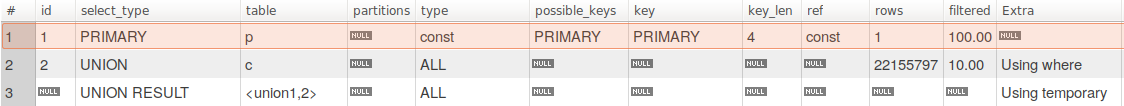
\includegraphics[scale =0.4]{explain8.png} 
	\caption{Przykład 2}
\end{figure}
\begin{spverbatim}
	SELECT * FROM Comments WHERE UserId = (SELECT id FROM Users WHERE DisplayName = 'Jarrod Dixon');
\end{spverbatim}
\begin{figure}[H]
	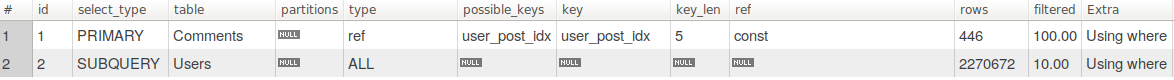
\includegraphics[scale =0.4]{explain9.png} 
	\caption{Przykład 3}
\end{figure}
\begin{spverbatim}
	SELECT * FROM Comments WHERE UserID in (SELECT UserId FROM Posts GROUP BY UserId HAVING COUNT(*) > 10);
\end{spverbatim}
\begin{figure}[H]
	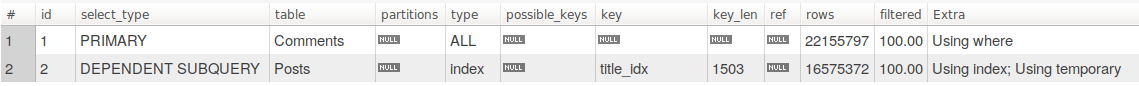
\includegraphics[scale =0.4]{explain9a.png} 
	\caption{Przykład 4}
\end{figure}
\begin{spverbatim}
	SELECT * FROM Comments WHERE UserID in (SELECT UserId FROM Posts GROUP BY UserId HAVING COUNT(*) > 10);
\end{spverbatim}
\begin{figure}[H]
	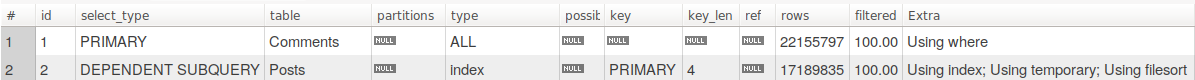
\includegraphics[scale =0.4]{explain10.png} 
	\caption{Przykład 5}
\end{figure}
\begin{spverbatim}
	SELECT * FROM Posts  WHERE OwnerUserId IN (SELECT id FROM Users WHERE Reputation>1000 UNION SELECT UserId FROM Comments WHERE Score >10)
\end{spverbatim}
\begin{figure}[H]
	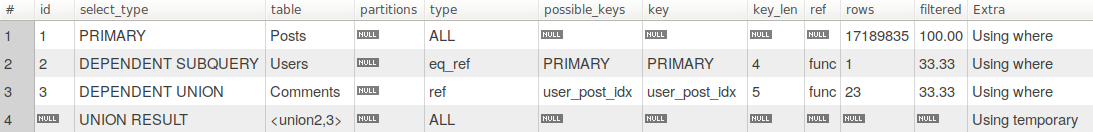
\includegraphics[scale =0.4]{explain11.png} 
	\caption{Przykład 6}
\end{figure}
\begin{spverbatim}
	SELECT * FROM Comments WHERE UserId = (SELECT @var1 FROM Users WHERE DisplayName = 'Jarrod Dixon');
\end{spverbatim}
\begin{figure}[H]
	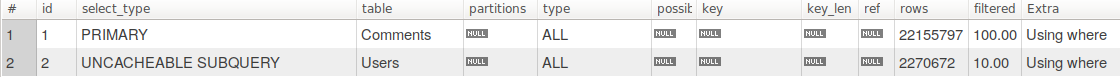
\includegraphics[scale =0.4]{explain12.png} 
	\caption{Przykład 7}
\end{figure}
\begin{spverbatim}
SELECT * FROM Comments LIMIT 10;
\end{spverbatim}
\begin{figure}[H]
	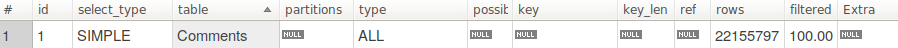
\includegraphics[scale =0.4]{explain13.png} 
	\caption{Przykład 8}
\end{figure}

\paragraph{Kolumna \#}
Wartości w kolumnie \# określają w jakiej kolejności MySQL będzie odczytywał tebele. Jako pierwsza odczytywana jest tabela z najmniejszą wartością.

\paragraph{Kolumna ID}\leavevmode\\
Kolumna id zawiera numer zapytania, którego dotyczy. W przypadku zapytań z podzapytaniami, podzapytania w dyrektywie FROM oraz zapytań z słowem kluczowym JOIN podzapytania numerowane są najczęściej względem ich występowania w zapytaniu. Kolumna ID może przyjąć również wartość NULL, w przypadku polecenia UNION (przykład 2).

\paragraph{Kolumna select\textunderscore type}\leavevmode\\
Kolumna select\textunderscore type pokazuje, czy rekord jest prostym, czy złożonym zapytaniem SELECT. 
Wartość \textbf{SIMPLE} oznacza, że zapytanie nie zawiera podzapytań, oraz nie używa klauzuli UNION.

Jeżeli natomiast zapytanie zawiera podzapytania lub wykorzystuje klauzulę UNION, to rekord dla kolumny select\textunderscore type przyjmie wartość \textbf{PRIMARY} (przykład 2). Jeżeli rekord dotyczy podzapytania oznaczonego jako PRIMARY, to będzie oznaczony jako \textbf{SUBQUERY} (przykład 3). Jako \textbf{UNION} zostaną oznaczone zapytania, które są drugim i kolejnym zapytaniem w klauzuli UNION. Pierwsze zapytanie zostanie oznaczone tak samo, jakby było wykonywane jako zwykłe zapytanie SELECT (przykład 2). \textbf{DERIVED} oznacza, że zapytanie jest umieszczone jako podzapytanie w klauzuli FROM, jest wykonywane rekurencyjnie i wyniki są umieszczane w tabeli tymczasowej. Wartość \textbf{UNION RESULT} oznacza wiersz, jako polecenie SELECT użyte do pobrania wyników z tabeli tymczasowej użytej przy poleceniu UNION (przykład 2). Jeśli polecenie SELECT zależy od danych znajdujących się w podzapytaniu lub znajdujących się w wyniki klazuli UNION, to zostanie oznaczone odpowiednio jako \textbf{DEPENDENT SUBQUERY} (przykład 5) lub \textbf{DEPENDENT UNION} (Przykład 6). Dodatkowo w przypadku, jeżeli wynik zwracany jest z \textit{zmaterializowanego widoku (eng. materialized view)}, zapytanie zostanie oznaczone jako \textbf{MATERIALIZED}. W przykładzie 7, który jest oczywiście nonsensowny, ale dobrze obrazuje sytuację, kiedy jako select\textunderscore type otrzymamy wartość \textbf{UNCACHABLE\textunderscore SUBQUERY}, która oznacza, że coś w podzapytaniu uniemożliwiło jego buforowanie. Analogiczną sytuację mamy, jeżeli wiersz zostanie oznaczony jako \textbf{UNCACHABLE\textunderscore UNION}, ale w tym przypadku niemożliwe jest oczywiście buforowanie wyników polecenia UNION.

\paragraph{Kolumna table}\leavevmode\\
Kolumna \textit{table} w większości przypadków zawiera nazwę tabeli lub jej alias, do której odnosi się dany wiersz wyniku polecenia \textit{EXPLAIN}. W przypadku gdy zapytanie dotyczy tabel tymczasowych możemy zobaczyć np. table: <union1,2> (przykład 2), co oznacza, że zapytanie dotyczy tabeli tymczasowej stworzonej na podstawie polecenia \textit{UNION} na tabelach z wierszy o id 1 oraz 2.
Odczytując kolejno wartości kolumny \textit{table} możemy dowiedzieć się, w jakiej kolejności optymalizator MySQL zdecydował się ułożyć zapytania. 

\paragraph{Kolumna Type}\leavevmode\\
Kolumna \textit{Type} informuje o tym, w jaki sposób MySQL będzie przetwarzał wiersze w tabeli. Poniżej przedstawiono najważniejsze metody dostępu do danych, w kolejności od najgorszej do najlepszej.

\subparagraph{ALL}\leavevmode\\
Wartość \textit{ALL} informuje o tym, że serwer musi przeskanować całą tabelę w celu odnalezienia rekordów. Istnieją jednak wyjątki takie, jak w przykładzie 8, w którym polecenie \textit{EXPLAIN} pokazuje, że będzie wykonywany pełny skan tabeli, a w rzeczywistości dzięki użyciu polecenia \textit{LIMIT} zapytanie będzie wymagało jedynie 10 rekordów.

\subparagraph{index}\leavevmode\\
MySQL skanuje wszystkie wiersze w tabeli, ale może wykonać to w porządku w jakim jest przechowywane w indeksie, dzięki czemu unika sortowania. Największą wadą jest jednak nadal konieczność odczytu całej tabeli. Co więcej, dane z dysku pobierane są z adresów, których kolejność wynika z użytego indeksu. Adresy te nie muszą zajmować na dysku ciągłych obszarów, a to oznacza, że czas odczytu danych może znacznie wydłużyć się. Jeżeli w kolumnie \textit{extra} jest dodatkowo zawarta informacja ''Using Index'' oznacza to, ze MySQL wykorzystuje indeks pokrywający (opisany w dalszej części pracy) i nie wymaga odczytywania innych danych z dysku – do wykonania zapytania wystarczają dane umieszczone w indeksie.

\subparagraph{range}\leavevmode\\
Wartość \textit{range} oznacza ograniczone skanowanie zakresu. Takie skanowanie rozpoczyna się od pewnego miejsca indeksu, dzięki czemu nie musimy przechodzić przez cały indeks. Skanowanie indeksu powodują zapytania zawierające klauzulę \textit{BETWEEN} lub \textit{WHERE} z < lub >. Wady są takie same jak przy rodzaju \textit{index}

\subparagraph{index\textunderscore subquery}\leavevmode\\
TODO przyklad
\subparagraph{unique\textunderscore subquery}\leavevmode\\
TODO przyklad
\subparagraph{index merge}\leavevmode\\
TODO przyklad
\subparagraph{fulltext}\leavevmode\\
TODO przyklad

\subparagraph{ref}\leavevmode\\
Jest to wyszukiwanie, w którym MySQL musi przeszukać jedynie indeks w celu znalezienia rekordu opowiadającego pojedynczej wartości.
Przykładem takiego zapytania może być wyszukiwanie numerów postów danego użytkownika w tabeli \textit{Comments} zawierającej indeks typu \textit{BTREE} na kolumnach \textit{UserId} oraz \textit{PostId}.

\begin{spverbatim}
	SELECT PostId FROM Comments WHERE UserId = 10;
\end{spverbatim}
Dodatkowo odmianą dostępu \textit{ref} jest dostępd \textit{ref\textunderscore or\textunderscore null}, który oznacza, że wymagany jest dodatkowy dostęp w celu sprawdzenia wartości NULL.


\subparagraph{eq\textunderscore ref}\leavevmode\\

Jest to najlepsza możliwa forma złączenia. Oznacza, że z tabeli odczytywany jest tylko jeden wiersz dla każdej kombinacji wierszy z poprzednich tabel. Z tego rodzaju złączeniem mamy do czynienia, jeżeli wszystkie kolumny używane do złączenia są kluczem głównym lub indeksem ''NOT NULL UNIQUE''. Przykładem takiego zapytania jest złączenie wszystkich komentarzy z postami bazując na kluczu głównym Id z tabeli Posts. 

\begin{spverbatim}
	SELECT * FROM Comments c JOIN Posts p ON c.PostId = p.id;
\end{spverbatim}

\subparagraph{const}\leavevmode\\
Przeważnie występuje w przypadku użycia w klauzuli WHERE wartości z indeksu głównego. Wtedy wystarczy jednokrotne przeszukanie indeksu, a na znalezionym liściu indeksu dostępne są już wszystkie dane z wiersza tabeli. Dla przykładu w bazie StackOverflow może to być zapytanie pobierające komentarz bazując na Id.
\begin{spverbatim}
	EXPLAIN SELECT * FROM Comments WHERE id = 93;
\end{spverbatim}

\subparagraph{NULL}\leavevmode\\
Oznacza, że serwer nie wymaga skanowania całej tabeli lub indeksu i może zwrócić wartość już podczas fazy optymalizacji. Przykładem takiego zapytania może być zwrócenie minimalnej wartości z indeksu tabeli.

\begin{spverbatim}
	SELECT MIN(UserId) FROM Comments;
	#Tabela Comments zawiera indeks BTREE na kolumnie UserID
\end{spverbatim}

\paragraph{Kolumna Possible\textunderscore keys}\leavevmode\\

Komulna possible\textunderscore keys zawiera listę indeksów, które optymalizator brał pod uwagę podczas tworzenia planu wykonania zapytania. Lista tworzona jest na początku procesu optymalizacji zapytania.

\paragraph{Kolumna key}\leavevmode\\

Kolumna \textit{key} sygnalizuje, który indeks został wybrany do optymalizacji dostępu do tabeli.

\paragraph{Kolumna key\textunderscore len}\leavevmode\\
Wartość oznacza jaki jest rozmiar bajtów użytego indeksu. W przypadku, kiedy zostanie wykorzystana jedynie część kolumn indeksu, wtedy wartość \textit{key\textunderscore len} będzie odpowiednio mniejsza. Istotny jest fakt, że rozmiar jest zawsze maksymalnym rozmiarem zindeksowanych kolumn, a nie rzeczywistą liczbą bajtów danych używanych do zapisu wiersza w tabeli.

\paragraph{Kolumna ref}\leavevmode\\
Kolumna pokazuje, które kolumny z innych tabel lub zmienne z innych tabel zostaną wykorzystane do wyszukania wartości w indeksie podanym w kolumnie \textit{key}. W przykładzie 1, widzimy, że do przeszukania indeksu tabeli Posts została wykorzystana kolumna UserId z tabeli Comments (alias c). Wartość \textit{const} oznacza, że do przeszukania wartości została wykorzystana stała podana np. w klauzuli WHERE (Przykład 2).

\paragraph{Kolumna rows}\leavevmode\\
Kolumna wskazuje oszacowaną liczbę wierszy, które MySQL będzie musiał odczytać w celu znalezienia szukanych rekordów. Wartość może znacząco odbiegać od rzeczywistej liczby wierszy, które zostaną odczytane podczas wykonania zapytania. Istotne jest to, że jest to liczba przeszukiwanych rekordów na danym poziomie zagnieżdenia pętli planu złączenia. To znaczy, że nie jest to całkowita liczba rekordów, a jedynie liczba rekordów w jednej pętli złączenia danej tabeli. W przypadku złączenia sumaryczna liczba przeszukiwanych nie jest sumą wartości z wszystkich wierszy, a iloczynem wartości z wierszy biorących udział w złączeniu. W przykładzie 9, łączna suma wierszy, które muszą zostać przeszukane nie wynosi 15748463.
\begin{spverbatim}
	SELECT * FROM Posts p JOIN PostTypes pt ON p.PostTypeId = pt.Id;
\end{spverbatim}
\begin{figure}[H]
	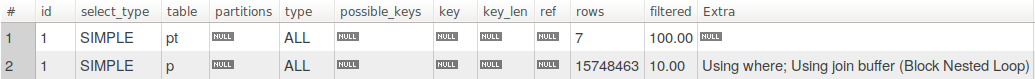
\includegraphics[scale =0.4]{explain14.png} 
	\caption{Przykład 9}
\end{figure}
Dodatkowo należy wziąć pod uwagę, że są to jedynie szacunkowe wartości, które w praktyce mogą być zupełnie nie prawidłowe. Ponadto optymalizator podczas szacowania wartości w kolumnie \textit{rows} nie bierze pod uwagę klauzli \textit{LIMIT}.

\paragraph{Kolumna filtered}\leavevmode\\
Kolumna \textit{filtered} pojawia się jedynie podczas użycia polecenia \textit{EXPLAIN EXTENDED}. Wskazuje na wartość oszacowaną przez optymalizator, która informuje ile rekordów może zostać odfiltrowane za pomocą klauzuli WHERE. W przykładzie 4 optymalizator MySQL oszacował, że jedynie 10 procent użytkowników napisało w sumie więcej niż 10 komentarzy. 

\paragraph{Kolumna extra}\leavevmode\\
Kolumna \textit{extra} zawiera informacje, których nie udało się zamieścić w pozostałych kolumnach. Poniżej przedstawione zostanie kilka najważniejszych informacji, które mogą znaleźć się w tej kolumnie.

\begin{itemize}
	\item 'Using index' - MySQL użyje indeksu pokrywającego zamiast dostępu do tabeli.
	\item 'Using where' - oznacza, że MySQL przeprowadzi filtrowanie danych dopiero po wczytaniu danych z tabeli. Często jest to informacja, która może sugerować zmianę lub stworzenia nowego indeksu bądź całego zapytania.
	\item 'Using temporary' - do sortowania wyników używana jest tabela tymczasowa.
	\item 'Using filesort' - sortowanie nie może skorzystać z istniejących indeksów (nie ma odpowiedniego optymalnego indeksu), więc wiersze są sortowane za pomocą jednego z algorytmów sortowania.
	
\end{itemize}
\section{Architektura MySQL}

\subsection{Obsługa połączeń i wątków}
Serwer MySQL oczekuje na połączenia klientów na wielu interfejsach sieciowych:
\begin{itemize}
\item jeden wątek obsługuje połączenia TCP/IP (standardowo port 3306)
\item w systemach UNIX, ten sam wątek obsługuje połączenia poprzez pliki gniazda
\item w systemie Windows osobny wątek obsługuje połączenia komunikacji międzyprocesorowej
\item w każdym systemie operacyjnym, dodatkowy interfejs sieciowy może obsługiwać połączenia administracyjne. Do tego celu może być wykorzystywany osobny wątek lub jeden z wątków menadżera połączeń.
\end{itemize}

Jeżeli dany system operacyjny nie wykorzystuje połączeń na innych wątkach, osobne wątki nie są tworzone.

Maksymalna ilość połączeń zdefinowana jest poprzez zmienną systemową \underline{max\_connections}, który domyślnie przyjmuje wartość 151. Dodaktowo MySQL jedno połączenie rezerwuje dla użytkownika z uprawnieniami \underline{SUPER} lub \underline{CONNECTION\_ADMIN}. Taki użytkownik otrzyma połączenie nawet w przypadku braku dostępnych połączeń w głównej puli.

Do każdego klienta łączącego się do bazy MySQL przydzielany jest osobny wątek wewnątrz procesu serwera, który odpowiada za przeprowadzenie autentykacji oraz dalszą obsługę połączenia. Co ważne, nowy wątek tworzony jest jedynie w ostateczności. Jeżeli to możliwe, menadżer wątków stara się przydzielić wątek do połączenia, z puli dostępnych w pamięci podręcznej wątków.

\subsection{Bufor zapytań}
Bufor zapytań przechowuje gotowe odpowiedzi serwera dla poleceń SELECT. Jeżeli wynik danego zapytania znajduje się w buforze zapytań, serwer może zwrócić wynik bez konieczności dalszej analizy.

Proces wyszukiwania zapytania w buforze wykorzystuje funkcję skrótu. Dla każdego zapytania tworzony jest hash, który pozwala w prosty sposób zweryfikować, czy dane zapytanie znajduje się w buforze. Co ważne, hash uwzględnia wielkość liter, co prowadzi do sytuacji, gdzie dwa zapytania różniące się jedynie wielkością liter nie zostaną uznane za jednakowe.

Jeżeli tabela, z której pobierane są dane poprzez polecenie SELECT  zostanie zmodyfikowana, wszystkie zapytania odnoszące się do takiej tabeli zostają usunięte z bufora. Dodatkowo bufor zapytań nie przechowuje zapytań uznanych, za niederministyczne. Przykładowo wszystkie polecenia pobierające aktualną datę, użytkownika itp nie zostaną dodane do bufora zapytań. Co istotne nawet w przypadku zapytania niederministycznego, serwer oblicza funkcję skrótu dla zapytania i próbuje dopasować odpowienie zapytanie z tabeli bufora. Dzieje się tak ze względu na fakt, że analiza zapytania odbywa się dopiero po przeszukaniu bufora i na etapie przeszukiwania bufora, serwer nie ma informacji o tym czy zapytanie jest deterministyczne. Jedynym filtrem, który weryfikuje zapytanie przed przeszukaniem bufora, jest sprawdzenie czy polecenie rozpoczyna się od liter SEL.

Jeżeli polecenie SELECT składa się z wielu podzapytań, ale nie znajduje się w tabeli bufora, to żadne z nich nie zostanie pobrane, ponieważ bufor zapytań działa na podstawie całego polecenia SELECT.



\section{Indeksy w MySQL}
Indeks jest strukturą danych zwiększającą szybkość operacji wyszukiwania na tabeli. Poprawne stosowanie indeksów jest krytyczne dla zachowania dobrej wydajności bazy danych.
Najprostszą analogią pozwalającą zrozumieć działanie indeksu w bazie danych jest porównanie go z indeksem znajdującym się w książce. Zakładając, że książka nie zawiera indeksu, wyszukiwanie konkretnego słowa lub tematu w najgorszym wypadku wymaga przewertowania całej książki. Z tego powodu w książkach stosuje się indeksy, które zawierają kluczowe słowa użyte w książce. Indeks taki zawiera listę słów oraz stron, na których słowa te występują. Dzięki temu wyszukanie konkretnego słowa wymaga jedynie sprawdzenia numeru strony w indeksie. Jest to szczególnie przydatne przy książkach zawierających dużą liczbę stron. Podobnie jest z tabelami w bazie danych. Przy tabelach o niewielkiej ilości wierszy, wyszukanie konkretnego rekordu trwa krótki nawet przy niestosowaniu indeksów. Indeksy stają się jednak kluczowe wraz ze wzrostem zbioru danych.
W MySQL istnieje wiele rodzajów indeksów, które są implementowane w wartstwie silnika bazy danych, dlatego też nie każdy rodzaj indeksu jest obsługiwany przez wszystkie silniki. W tym rozdziale omówię tylko najpopularniejsze z nich.
\subsection{Indeksy typu B-Tree}
Indeks typu B-Tree jest zdecydowanie najczęściej stosowanym typem indeksu w bazach MySQL i jest domyślnie wybierany przez serwer MySQL podczas tworzenia nowego indeksu. Dlatego właśnie jemu poświęce zdecydowaną wiekszość tego rozdziału.

\paragraph{Struktura}\mbox{}

Indeks typu B-Tree zbudowany jest na bazie struktury B-Drzewa. B-Drzewo jest drzewiastą strukturą danych przechowującą dane wraz z kluczami posortowanymi w pewnej kolejności. Każdy węzeł drzewa może posiadać od M+1 do 2M+1 dzieci, za wyjątkiem korzenia, który od 0 do 2M+1 potomków, gdzie M jest nazywany rzędem drzewa. Dzięki temu maksymalna wysokość drzewa zawierającego n kluczy wynosi $log_M n$. Takie właściwości sprawiają, że operacje wyszukiwania są złożoności asymptotycznej $O(log_M n)$. Chcąc być dokładnym, należy wspomnieć, że MySQL do zapisu indeksów stosuje strukurę B+Drzewa, która jest szczególnym przypadkiem B-Drzewa i zawiera dane jedynie w liściach.
Zastosowanie struktury B+Drzewa sprawia, że liście z danymi znajdują się w jednakowej odległości od korzenia drzewa. Wysoki rząd oznacza niską wysokość drzewa, to z kolei sprawia, że zapytanie wymaga mniejszej ilości operacji odczytu z dysku. Ma to fundamentalne znaczenie, ponieważ dane zapisane są na dyskach twardych, których czasy dostępu są dużo większe niż do pamięci RAM. Dla przykładu, załóżmy, że dana jest tabela zawierająca bilion wierszy, oraz indeks, którego rząd wynosi 64. Operacja wyszukania na danej tabeli wykorzystująca indeks będzie wymagać średnio tylu operacji odczytu, jaka jest wysokość drzewa przechowującego indeksy. Wysokość drzewa obliczamy ze wzoru $\log M n$,gdzie M jest rzędem drzewa równym 64, a n oznacza ilość wierszy. W takim przypadku będziemy potrzebować zaledwie 5 odczytów danych z dysku. Dodatkowo silnik InnoDB nie przechowuje referencji do miejsca w pamięci, w którym znajdują się dane, ale odwołuje się do rekordów poprzez klucz podstawowy, który jednoznacznie identyfikuje każdy wiersz w tabeli.Dzięki temu zmiana fizycznego położenia rekordu nie wymusza aktualizacji indeksu. Indeksy mogą być zakładane zarówno na jedną jak i wiele kolumn. W przypadku indeksu wielokolumnowego, węzły sortowane są w pierwszej kolejności względem pierwszej kolumny indeksu. W następnej kolejności węzły z równymi wartościami pierwszej kolumny, sortowane są względem drugiej itd. Kolejność kolumn jest ustalana na podstawie kolejności podczas polecenia tworzenia indeksu.

\paragraph{Zastosowanie indeksu typu B-Tree}\mbox{}

Aby przedstawić działanie indeksu typu B-Tree na rzeczyczywistym przykładzie przygotowałem dwie tabele. Pierwszą jest tabela \textit{Comments} z bazy danych stackoverflow. Drugą tabelą jest \textit{Init\textunderscore Comments}, która jest kopią tabeli Comments i nie zawiera klucza głównego oraz indeksów.
Dla tabeli \textit{Comments\textunderscore idx} za pomocą polecania \begin{verbatim}
    CREATE INDEX user_post_idx 
ON Comments(UserId,PostId);
\end{verbatim}
utworzyłem indeks typu B-Tree na dwóch kolumnach \textit{first\textunderscore UserId} oraz \textit{last\textunderscore PostId}.

\subparagraph{Dopasowanie pełnego indeksu}\mbox{}

Załóżmy, że w tabeli \textit{Comments} chcemy wyszukać wszystkie komentarze użytkownika o id 1200 do postu o id 910331.

Najpierw wykonamy zapytania na tabeli nie zawierającej indeksów.
 \textit{employees}. 
\begin{verbatim}
    SELECT * FROM Init_Comments WHERE UserId = 1200 AND PostId = 910331;
\end{verbatim}
Zapytanie zwróciło wynik w 13,7 sekundy.

Następnie analogiczne zapytanie wykonałem na tabeli \textit{Comments} zawierającej indeks na obu kolumnach.
\textit{employees\textunderscore idx}. 
\begin{verbatim}
    SELECT * FROM Comments WHERE UserId = 1200 AND PostId = 910331;
\end{verbatim}
Tym razem zapytanie zwróciło wyniki w 0,013 sekundy. Tym razem serwer nie skanował całej tabeli. Z czego wynika różnica w czasie wykonania obu zapytań? Wykorzystując polecenie EXPLAIN dla obu zapytań otrzymujemy ciekawe dane. Rysunek 2 przestawia wynik polecenia EXPLAIN dla pierwszego zapytania, natomiast Rysunek 3 wynik polecania EXPLAIN dla drugiego zapytania. Polecenie EXPLAIN wyjaśnia, że pierwsze zapytania nie będzie korzystać z indeksów, dlatego w kolumnie rows widzimy, że serwer MySQL będzie musiał przeskanować wszystkie 23 miliony wierszy z tabeli \textit{init\textunderscore Comments}. Drguie zapytanie korzysta z indeksu z naszego indeksu. Tym razem serwer będzie musiał przeskanować jedynie 3 wiersze tabeli Comments. 

\begin{figure}[h]
    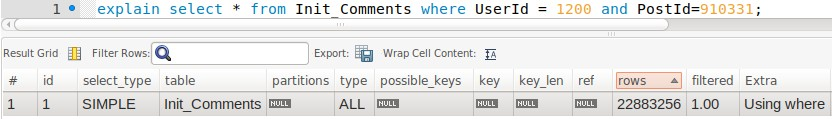
\includegraphics[scale =0.5]{explain1.jpg} 
    \caption{EXPLAIN 1}
\end{figure}

\begin{figure}[h]
    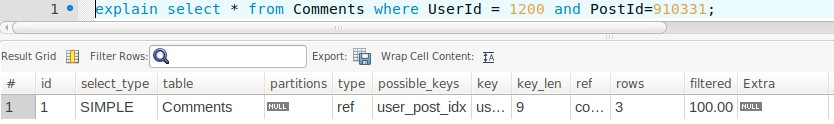
\includegraphics[scale =0.5]{explain2.jpg} 
    \caption{EXPLAIN 2}
\end{figure}

Dopasowanie pełnego indeksu ma miejsce wtedy, kiedy w klauzuli \textit{where} uwzględnimy wszystkie kolumny, na które założony jest indeks. 
\subparagraph{Dopasowanie prefiksu znajdującego się najbardziej na lewo}\mbox{} 
Dopasowanie prefiksu znajdującego się najbardziej na lewo może pomóc w wyszukaniu wsystkich komentarzy użytkownika. Załóżmy, że chcemy znaleźć wszystkie komentarze użytkownika o id 1200.
W tym celu przygotowujemy dwa zapytania. Pierwsze na tabeli \textit{Init\textunderscore Comments}, drugie na tebeli \textit{Comments} zawierającej indeks typu B-Tree, który założyliśmy wcześniej.
\begin{verbatim}
    SELECT * FROM Init_Comments WHERE UserId = 1200;
\end{verbatim}
\begin{verbatim}
    SELECT * FROM Comments WHERE UserId = 1200;
\end{verbatim}
Pierwsze zapytanie zostało wykonane w czasie 12,9 sekundy, natomiast drugie wymagało jedynie 0,0044 sekundy. Ponownie sprawdźmy rezultat polecenia EXPLAIN na obu zapytaniach. W pierwszym zapytaniu serwer po raz kolejny musiał przeszukać wszystkie wiersze w tabeli. Drugie zapytanie wymagało przeszukania 209 wierszy, dlatego że tym razem zapytanie było mniej selektywne niż przy dopasowaniu pełnego indeksu.
\begin{figure}[h]
    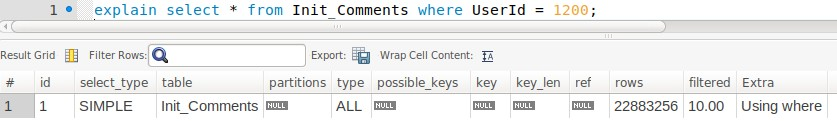
\includegraphics[scale =0.5]{explain3.jpg} 
    \caption{EXPLAIN 3}
\end{figure}

\begin{figure}[h]
    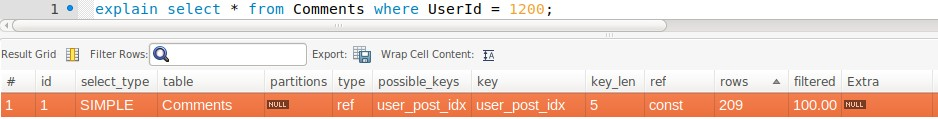
\includegraphics[scale =0.5]{explain4.jpg} 
    \caption{EXPLAIN 4}
\end{figure}

\subparagraph{Dopasowanie zakresu wartości}\mbox{}
Dopasowanie zakresu wartości oznacza wyszukiwanie wartości w danym przedziale. W naszym przypadku może to być wyszukiwanie wszystkich komentarzy użytkowników o identyfikatorach z przedziału od 1990 do 2000.

Ponownie wykonujemy dwa zapytania. Pierwsze na tabeli bez indeksu, drugie na tabeli z indeksem.
\begin{verbatim}
    SELECT * FROM Init_Comments WHERE UserId >1990 AND UserId <2000;
\end{verbatim}

Tym razem pierwsze zapytanie trwało 1.068 sekundy. Drugie zapytanie wykonujemy na tabeli Comments zawierającej indeksy.
\begin{verbatim}
    SELECT * FROM Comments WHERE UserId >1990 AND UserId <2000;
\end{verbatim}
Następnie sprawdzamy wynik polecenia EXPLAIN dla obu zapytań. Przy pierwszym zapytaniu, kolejny raz MySQL przeskanował całą tabelę Init\textunderscore Comments. Drugie natomiast wymagało przeskanowania jedynie wierszy, które zostały zwrócone jako rezultat zapytania.

\begin{figure}[h]
    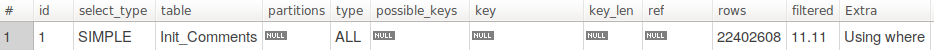
\includegraphics[scale =0.5]{explain5.png} 
    \caption{EXPLAIN 5}
\end{figure}

\begin{figure}[h]
    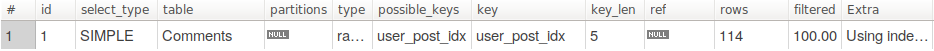
\includegraphics[scale =0.5]{explain6.png} 
    \caption{EXPLAIN 6}
\end{figure}


PREFIX INDEX
będą wymagały przeszukania całej tabeli. Dodatkowo wyszukiwanie za pomocą prefiksu nie będzie optymalne w przypadku indeksu wielokolumnowego dla wszystkich kolumn z wyjątkiem pierwszej. Jest to bezpośrednim następstwem budowy indeksów typu B-Tree i wynika z faktu sortowania kluczy względem pierwszej kolumny.





\subparagraph{Zapytania dotyczące jedynie indeksów}\mbox{}
Zapytania dotyczące jedynie indeksów to zapytania, które wykorzystują jedynie wartości indeksu, a nie do rekordów bazy danych.





 
Indeks jednokolumnowy zawiera klucze posortowane zgodnie z wartościami kolumny, na której założony został indeks. W przypadku indeksów wielokolumnowych węzły sortowane są w kolejności kolumn w indeksie. Zakładając, że indeks został założony na kolumnach k1,k2 oraz k3, dane w pierwszej kolejności zostaną posortowane zgodnie z wartościami kolumny k1. Następnie rekordy z równą wartością kolumny k1 zostaną posortowane zgodnie z wartościami kolumny k2. Analogicznie rekordy z równą wartością kolumny k1 oraz k2 zostaną posortowane zgodnie z wartościami kolumny k3. Zrozumienie tej zasady jest kluczowe do poprawnego korzystania z indeksów typu B-Tree. Taka struktura powoduje, że taki indeks jest użyteczny tylko w przypadku, gdy wyszukiwanie używa znajdujego się najbardziej na lewo prefiksu indeksu.
Kolejnym zastosowaniem indeksu typu B-Tree jest wyszukiwanie na podstawie prefiksu kolumny. Przykładem takiego zapytania może być wyszukiwanie wszystkich pracowników, których nazwiska rozpoczynają się od litery K (zakładamy, że tabela posiada indeks na kolumnie nazwisko). Istotnym jest fakt, że indeks staje się nieprzydany przy wyszukiwaniu na podstawie suffixu lub środkowej wartości. Następnym przypadkiem, w którym indeks typu B-Tree przyśpiesza zapytanie, jest wyszukiwanie na podstawie zakresu wartości. Dla tabeli z indeksem typu B-Tree założonym na kolumnie k, indeks może posłużyć do efektywnego wyszukania wartości z przedziału wartości tej kolumny. Zastosowanie struktury B-Tree powoduje, że sortowanie wyników zapytania względem indeksy jest zdecydowanie bardziej wydajne.


\subsection{Indeksy typu hash}
Indeksy typu hash są dostępne jedynie dla tabel silnika \textit{MEMORY} i są domyślnie ustawianymi indeksami dla takich tabel. Indeksy typu \textit{hash} opierają się na funkcji skrótu liczonej na wartościach indeksowanych kolumn. Dla każdego rekordu takiej tabeli liczona jest krótka sygnatura, na podstawie wartości klucza wiersza. Podczas wyszukiwania wartości na podstawie kolumn indeksowanych tego typu kluczem obliczana jest funkcja skrótu dla klucza, a następnie wyszukuje w indeksie odpowiadających wierwszy. Możliwe jest, że do jednej wartości funkcji skrótu dopasowane zostanie więcej niż jeden różny wiersz. Takie zachowanie wynika bezpośrednio z zasady działania funkcji skrótu, która nie zapewnia unikatowości dla różnych wartości dla zbioru danych wejściowych. Niemniej taka sytuacja nie należy do częstych i nawet wtedy operacja wyszukiwania na podstawie indeksu typu hash jest bardzo wydajna, ponieważ serwer w najgorszym wypadku musi odczytać zaledwie kilka wierszy z tabeli. Stąd wynika największa zaleta indeksów typu \textit{hash} w stosunktu do indeksów \textit{B-Tree}; czas wyszukiwania dowolnego wiersza w tabeli jest stały niezależnie od liczby wierszy. Podstawową wadą indeksu typu hash jest konieczność wyszukiwania na podstawie pełnej wartości klucza. Wynika to z tego, że funkcja skrótu wyliczona na podstawie niepełnego zbioru danych, nie ma korelacji z wartością funkcji wyliczonej na pełnym kluczu. Dodatkowo indeksy hash nie optymalizują operacji sortowania, ponieważ wartości funkcji f1, f2 skrótu dla dwóch rekordów x1 oraz x2, gdzie x1 jest mniejsze od x2 nie zapewniają, że f1 będzie mniejsze od f2. Dodatkowo z racji ograniczonego zbioru wartości funkcji hashującej, mogą występować problemy ze skalowaniem w przypadku dużych zbiorów danych. Po przekroczeniu pewnej liczby wierszy, należy zwiększyć rozmiar klucza indeksu i ponownie obliczyć funkcję dla wszystkich wierszy w tabeli.


\end{document}